\documentclass[compress]{beamer}
\usepackage[utf8x]{inputenc}
\usepackage{default}
\usepackage{graphics}
\usepackage{ulem}
\usepackage{multicol}

\useinnertheme{rounded}
\usecolortheme{whale}
\useoutertheme[subsection=false]{miniframes}
\setbeamertemplate{footline}[frame number]
\beamertemplatenavigationsymbolsempty

%%%%%%%% begin tikz %%%%%%
\usepackage{tikz}
\usetikzlibrary{shapes.callouts,decorations.pathmorphing}
\usetikzlibrary{shapes,decorations,shadows}
\usetikzlibrary{decorations.pathmorphing}
\usetikzlibrary{decorations.shapes}
\usetikzlibrary{fadings}
\usetikzlibrary{patterns}
\usetikzlibrary{calc}
\usetikzlibrary{decorations.text}
\usetikzlibrary{decorations.footprints}
\usetikzlibrary{decorations.fractals}
\usetikzlibrary{shapes.gates.logic.IEC}
\usetikzlibrary{shapes.gates.logic.US}
\usetikzlibrary{fit,chains}
\usetikzlibrary{positioning}
\usepgflibrary{shapes}
\usetikzlibrary{scopes}
\usetikzlibrary{arrows}
\usetikzlibrary{backgrounds}


\pgfdeclarelayer{background}
\pgfdeclarelayer{foreground}
\pgfsetlayers{background,main,foreground}

\tikzset{latent/.style={circle,fill=white,draw=red,thick,inner sep=1pt, 
minimum size=20pt, font=\fontsize{10}{10}\selectfont},
obs/.style={latent,fill=gray!25},
const/.style={rectangle, inner sep=0pt},
factor/.style={rectangle, fill=red,minimum size=7pt, inner sep=0pt},
yellow/.style={latent,minimum size=15pt,fill=yellow!75},
blue/.style={latent,minimum size=15pt,fill=blue!75},
-/.style={color=red, thick},
>={triangle 45}}




% shapename, fitlist, caption, pos
\newcommand{\plate}[4]{
\node (invis#1) [draw, transparent, inner sep=1pt,rectangle,fit=#2] {};
\node (capt#1) [ below left=0 pt of invis#1.south east, xshift=0pt,yshift=-9pt] {\raisebox{0pt}[0pt]{\footnotesize{#3}}};
\node (#1) [draw=black!50,thick,inner sep=3pt,rectangle,rounded corners,fit=(invis#1) (capt#1),#4] {};
}


\newcommand{\shiftedplate}[5]{
\node (invis#1) [draw, transparent, inner sep=0 pt,rectangle,fit=#2] {};
\node (capt#1) [#5, xshift=2pt] {\footnotesize{#3}};
\node (#1) [draw,inner sep=2pt, rectangle,fit=(invis#1) (capt#1),#4] {};
}
%shapename, pos, caption, in, out, captpos
\newcommand{\factor}[6]{
\node (#1) [factor] at #2 {};
\node (capt#1) [#6 of #1]{\footnotesize{#3}};
\draw [-] (#4) -- (#1) ;
\draw [->,thick] (#1) -- (#5);
}

% name, --, caption, pos
\newcommand{\nofactor}[4]{
\node (#1) [factor, #2]  {};
\node (capt#1) [#4 of #1]{\footnotesize{#3}};
}


\title{Novelty Detection Using Graphical Models for
       Semantic Room Classification}
\author{André Susano Pinto\inst{1,2} \and Andrzej Pronobis\inst{1} \and Luis Paulo Reis\inst{2}}
\date{18 July 2011}

\institute {
 \inst{1}The Royal Institute of Technology (KTH), Sweden \\
 \inst{2}Faculdade de Engenharia da Universidade do Porto
}

\begin{document}
\begin{frame}
 \titlepage
\end{frame}

\section{Summary}
\begin{frame}{Summary - Plan}
    \begin{block}{Semantic mapping of indoor enviroments}
        \begin{itemize}
            \item What is it? What for?
            \item How to, using graphical models
            \item Limited on the agent knowledge of variable categories
        \end{itemize}
    \end{block}
    \begin{block}{Novelty Detection}
        \begin{itemize}
            \item Trigger on $P(x|known)$
            \item Dynamic graphs
            \item $P(x|known)/P(x)$
            \item Approximating $P(x)$
        \end{itemize}
    \end{block}
\end{frame}

\begin{frame}{Goals}
  Brief introduction
  \begin{itemize}
    \item Study a semantic mapping process in the context of mobile robots.
    \item Propose a method based on the studied system to detect novel semantic categories of places.
  \end{itemize}
\end{frame}

\begin{frame}{Outline}
  \begin{multicols}{2}
    \tableofcontents
  \end{multicols}
\end{frame}


\section{Semantic Mapping}
\subsection{Introduction}
\begin{frame}{Semantic Mapping}
    \begin{columns}[tt]
        \column{0.5\textwidth}
        \begin{figure}
            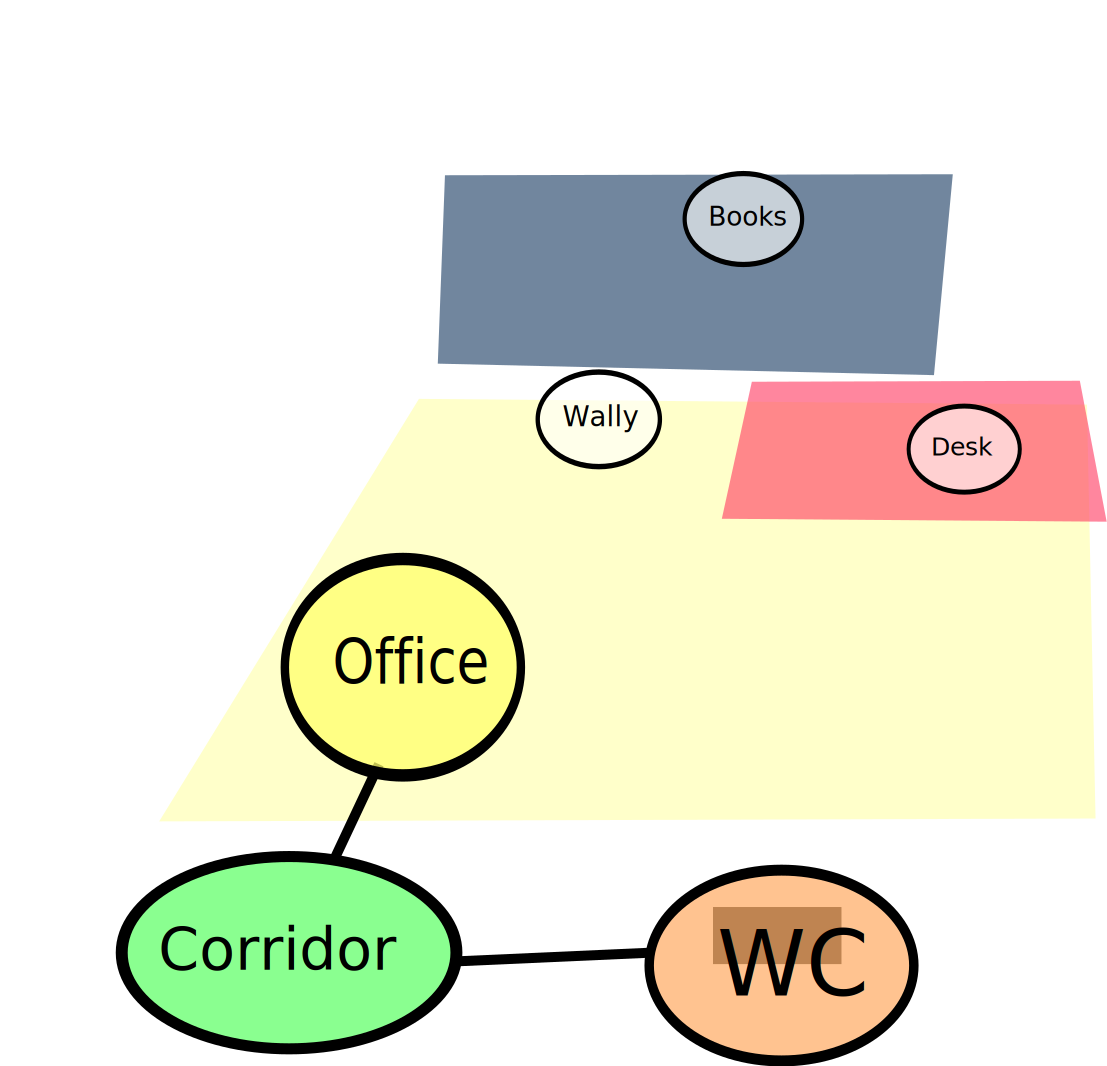
\includegraphics[width=\textwidth]{figures/semanticfriendly.pdf}
        \end{figure}

        \column{0.5\textwidth}
\only<1>{
        \begin{block}{Use of Human Semantics}
            Expanding space representation with semantics. 
        \end{block}
        \begin{block}{Focus on Room Categories}
            Semantic categories help describing expected properties and functionality.
        \end{block}
}
\only<2>{
        \begin{figure}
            \begin{tikzpicture}
                \node (human) at (0,0) {\reflectbox{
\includegraphics[width=0.4\textwidth]{figures/extra/bart.pdf}}};
                \node (robot) at (3,0) {\reflectbox{\includegraphics[width=0.2\textwidth]{figures/robot.png}}};

                \node[ellipse callout, draw, callout absolute pointer={(human.70)}]
                (humanvoice) at (1,3) {Where is Wally?};

                \node[ellipse callout, draw, callout absolute pointer={(robot.north)},
                text width=0.2\textwidth]
                (robotvoice) at (3,2) {In the office};

            \end{tikzpicture}
        \end{figure}
}
    \end{columns}
\end{frame}

\subsection{Dora Architecture Overview}
\begin{frame}{Dora Architecture Overview}
    \begin{block}{Multi-modal approach}
        Combining semantic data extracted from diferent sources is expected to yield better performance.
    \end{block}
    \begin{block}{Probabilistic approach}
        TODO: Need to defend use of probabilistic approach and graphical models.
    \end{block}
\end{frame}

\begin{frame}{Dora Architecture Overview}
  \begin{figure}
    \includegraphics[width=0.8\textwidth]{figures/processes.pdf}
  \end{figure}
\end{frame}

\subsection{Spatial Knowledge and Conceptual Map}
\begin{frame}{Spatial Knowledge and Conceptual Map}
  \begin{columns}[c]
  \column{0.5\textwidth}
    \begin{figure}
      \includegraphics[width=\textwidth]{figures/chaingraph.pdf}
    \end{figure}
  \column{0.5\textwidth}
    \begin{block}{Conceptual Map}
      The ontology is used to identify instances of the concepts and categories
      and perform probabilistic semantic mapping using graphical models.
    \end{block}
  \end{columns}
\end{frame}

\subsection{Graphical Models}
\begin{frame}{Graphical models}
    Multi-modal probabilistic semantic mapping using graphical models.
    Uncertain semantic information
    Conceptual map
    Probabilistic inference on variables

            $\text{known} = \{\text{corridor}, \text{office}, \cdots\}$
            $R_i \in \text{known}$

    TODO: picture explaining that maybe roomA is not known and showing X (observed features) and introduced novel and not novel, and showing graph structure.

\end{frame}

\section{Novelty Detection}
\subsection{Introduction}
\begin{frame}{Novelty Detection}
    \begin{columns}[c]
        \column{0.5\textwidth}
        \centering
        \includegraphics[width=\textwidth]{figures/conditional-prob-graph.pdf}

        \column{0.5\textwidth}
        \only<1>{
        \begin{itemize}
            \item Deploy on new and unknown environments
            \item Active-learning and self-extension
            \item Detect Knowledge-Gaps
        \end{itemize}
        }
        \only<2>{
        \begin{block}
            {Novel room category?}
            \begin{itemize}
                \item Detect \alert{$R_1\notin \text{known}$}
            \end{itemize}
        \end{block}
        }
    \end{columns}
\end{frame}


\subsection{Novelty Detection via Thresholding}
\begin{frame}
    $\frac{P(x|\overline{novel})P(\overline{novel})}{P(x)} \propto \frac{P(x|\overline{novel})}{P(x)} \propto P(x|\overline{novel})$
    \begin{block}{$P(novel)$ constant}
        Warning: assuming any graph structure has the same probability of generating
        novel classes.
    \end{block}
    \begin{block}
        Assumption on uniform $P(x)$.
    \end{block}
\end{frame}


\subsection{Dynamic distributions}
\begin{frame}
    The set of observed features and graph structure is always changing.
    Threshold on $P(x|known)$ \cite{bishop1994novelty}
    Dynamic graphs
\end{frame}

\subsection{Semi-supervised}
\begin{frame}
    
\end{frame}

\subsection{Results}
\begin{frame}
    Synthetic dataset where 1 room category is responsible for generating a variable set of observed features.
\end{frame}

\section{Conclusion}
\subsection{Conclusion}
\begin{frame}
    \begin{block}
        {Semantic Mapping Process}
        A multi-modal semantic mapping process based on \emph{probabilistic graphical models}.
    \end{block}
    \begin{block}
        {Novelty detection via thresholding}
        Presented a method to detect novel classes on a variable of \emph{probabilistic graphical models}
        dinamicaly instatiated from sensed semantic data.
    \end{block}
\end{frame}

\subsection{Future Work}
\begin{frame}{Future Work}
    \begin{block}
        {Incorporate novelty signals}
    \end{block}
\end{frame}




\appendix
% \begin{frame}[allowframebreaks]{Bibliography}
% \bibliographystyle{alpha}
% \bibliography{refs}
% \end{frame}
% 
\begin{frame}
 \titlepage
\end{frame}

\end{document}

